 \section{Stochastic chemical kinetics}
\label{app:coeffs}
 
 In this section we briefly describe how reaction and diffusion events
are modeled and how we obtain the diffusion rate constants when the
domain is discretized using an unstructured mesh. For a more detailed
introduction to the subject along with many additional references,
consult e.g. \cite{stefan_phd}.

The computational core of URDME is based on the next subvolume method
(NSM) \cite{BISTAB}. Details
concerning the actual simulation algorithms can be found in
Appendix~\ref{app:algorithms}.


\subsection{Mesoscopic chemical kinetics}

In a well-stirred chemical environment reactions are understood as
transitions between the states of the integer-valued state space
counting the number of molecules of each of $D$ different species. The
intensity of a transition is described by a \emph{reaction propensity}
defining the transition probability per unit of time for moving from
the state $x$ to $x+N_r$;
\begin{align}
  \label{eq:prop}
  x &\xrightarrow{\omega_{r}(x)} x+N_{r},
\end{align}
where $N_{r} \in \mathbf{Z}^{D}$ is the transition step and is the
$r$th column in the \emph{stoichiometric matrix}
$N$. Eq.~\eqref{eq:prop} defines a continuous-time Markov chain over
the positive $D$-dimensional integer lattice.

When the reactions take place in a container of volume $\Omega$, it is
sometimes useful to know that the propensities often satisfy the
simple scaling law
\begin{align}
  \omega_{r}(x) &= \Omega u_{r}(x/\Omega)
\end{align}
for some function $u_{r}$ which does not involve $\Omega$. Intensities
of this form are called \emph{density dependent} and arise naturally
in a variety of situations \cite[Ch.~11]{Markovappr}.

\subsection{Mesoscopic diffusion}
\label{subsec:mesodiff}

In the mesoscale model, a diffusion event is modeled as a first order
reaction taking species $S_l$ in subvolume $\zeta_i$ from its present
subvolume to an adjacent subvolume $\zeta_j$,
\begin{equation}
  S_{li} \xrightarrow{a_{ij}\fatx_{li}} S_{lj},
\end{equation}        
where $\fatx_{li}$ is the number of molecules of species $l$ in
subvolume $i$. On a uniform Cartesian mesh such as those used in
MesoRD \cite{mesoRD}, the rate constant takes the value $a_{ij}=\gamma
/h^2$ where $h$ is the side length of the subvolumes and $\gamma$ is
the diffusion constant. In URDME we use an unstructured mesh made up
of tetrahedra and the rate constants are taken such that the expected
value of the number of molecules divided by the volume (the
concentration) converges to the solution obtained from a consistent
FEM discretization of the diffusion equation
\begin{equation}
  u_t = \gamma \Delta u.
\end{equation}
Using piecewise linear Lagrange elements and mass lumping, we obtain
the discrete problem
\begin{equation}
  \label{eq:FEM}
  u_t = M^{-1}Ku
\end{equation}
where $M$ is the lumped mass matrix and $K$ is the
stiffness matrix. The rate constants on the unstructured mesh are then
given by
\begin{equation}
  a_{ij} = \frac{1}{\Omega_i} k_{ij}, 
\end{equation}
where $\Omega_i$ is the diagonal entry of $M$ and can be interpreted
as the volume of the dual element associated with mesh node $i$ (see
Figure~\ref{fig:dual}). For more details, consult
\cite{SPDEPEFHL}.

\begin{figure}[htb!]
  \centering  
  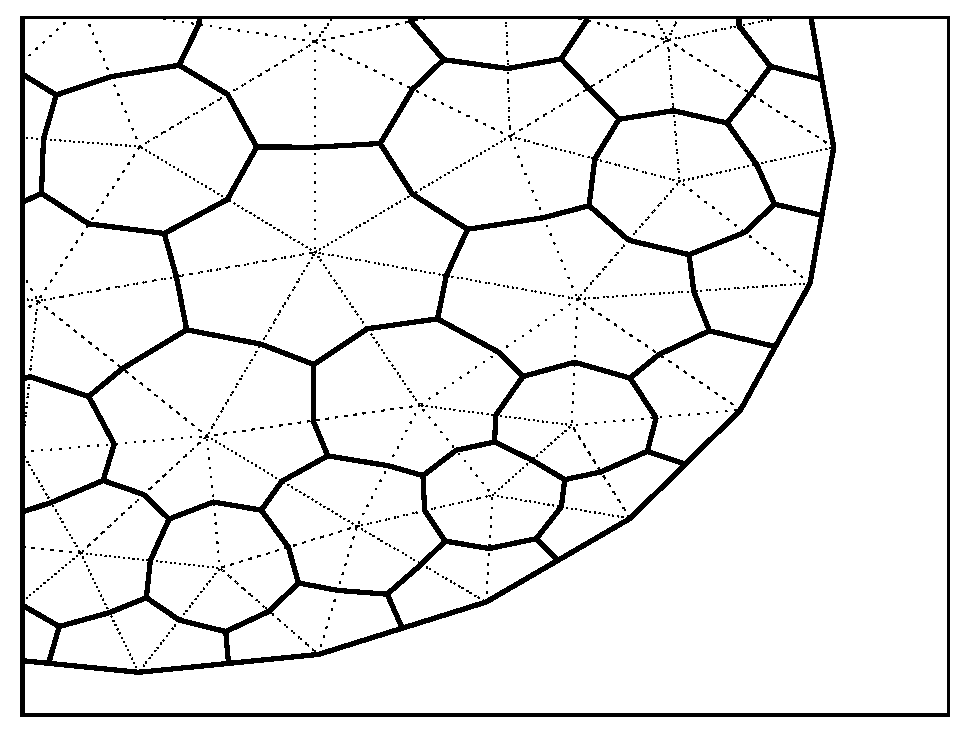
\includegraphics[width=0.6\linewidth,height=0.6\linewidth]
    {fig/URDMEmesh}
  \caption{A 2D example of an unstructured triangular mesh. The primal
  mesh is shown in dashed and the dual in solid. Within each dual
  element the system is assumed to be well-stirred, and molecules can
  jump from each dual cell to the neighboring ones.}
  \label{fig:dual}
\end{figure}

The assumption made in the mesoscopic model is that molecules are
well-stirred within a dual cell. These dual cells correspond to the
cubes of the staggered grid in a Cartesian mesh.
